\apendice{Documentación técnica de programación}

\section{Introducción}

\section{Estructura de directorios}

En la figura~\ref{fig:directorios} se muestra la estructura de directorios del repositorio de GitHub en el que se encuentra alojado el proyecto: \url{https://github.com/aog0036/TFG-SmartBeds}. 

El contenido del repositorio se estructura principalmente en tres directorios: 
\begin{itemize}
	\item \textbf{/android:} Contiene el proyecto de Android Studio con los ficheros de código fuente, los de test, los de configuración y el fichro .apk generado. 
	\item \textbf{/doc:} Contiene la documentación general del proyecto, incluyendo la memoria, los anexos y el cuaderno de investigación, todos en formado .pdf y en formato .tex. También contiene otros recursos como las imágenes y los archivos con las referencias bibliográficas (extensión .bib). 
	\item \textbf{/jupyter notebooks:} Contiene los notebooks y los scripts de python con los experimentos generados durante la fase de investigación. 
\end{itemize}

Dentro del proyecto de Android Studio los directorios más importantes son los siguientes: 
\begin{itemize}
	\item \textbf{/app:} Contiene los directorios release, src y los que contienen los ficheros de pruebas unitarias y de interfaz. 
	\item \textbf{/app/release:} Contiene el fichero SmartBeds.apk para la instalación y distribución de la aplicación en un dispositivo Android. 
	\item \textbf{/app/src/main/java/.../smartbeds:} Contiene los paquetes con las clases Java que componen el código fuente de la aplicación. 
	\item \textbf{/app/src/main/res:} Contiene los directorios con los archivos .xml que definen los recursos gráficos de la aplicación (interfaces, colores, menús...). 
	\item \textbf{/app/src/main/AndroidManifest.xml:} Manifiesto que contiene información esencial sobre la aplicación y que permite al sistema ejecutarla. 
	\item \textbf{/app/src/androidTest/.../generalActivities:} Contiene las pruebas de interfaz gráfica generadas mediante la herramienta Espresso. 
	\item \textbf{/app/src/test/.../smartbeds:} Contiene las pruebas unitarias generadas mediante JUnit. 
	\item \textbf{/javadoc:} Contiene la documentación de las clases y métodos del código de la aplicación en formato html. 
	\item \textbf{archivos de configuración de gradle:} Son una serie de directorios y ficheros generados automáticamente por Android Studio y que permiten construir la aplicación con la configuración y las dependencias necesarias. 
\end{itemize}

\begin{figure}
	\centering
	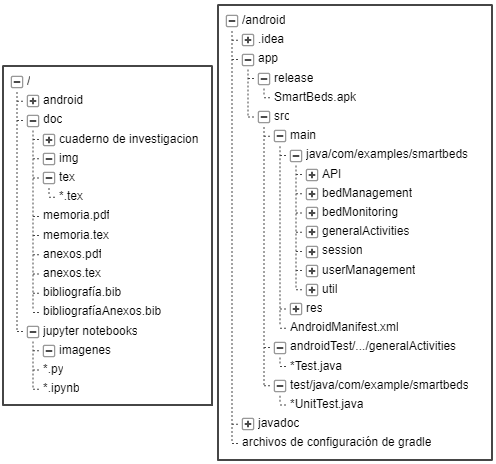
\includegraphics[width=1\textwidth]{../img/directorios.png}
	\caption{Estructura de directorios del repositorio.}
	\label{fig:directorios}
\end{figure}

\section{Manual del programador}

\section{Compilación, instalación y ejecución del proyecto}

\section{Pruebas del sistema}
